A simple pendulum consists of a small object (known as the bob) suspended from an inextensible string of negligible mass. When left undisturbed the bob hangs motionless with the string vertical. If the bob is pulled to one end and let go it begins to swing back and forth.

\section{Experimental Setup}

   \tikzsetnextfilename{setup}
\begin{center}
   \begin{tikzpicture}

      \usetikzlibrary{patterns}
      % We define a tikz style which defines a fill pattern consisting of lines in the north east direction.
      % The draw=none option indicates that we do NOT want any stroke/border around the fill
      \tikzstyle{wall}=[fill,pattern=north east lines,minimum width=0.75cm,minimum height=0.3cm, draw=none]


      % Define dimensions and angles
      \def\hw{0.25}     % Half width of the small wall segment on top

      \def\angle{-120}  % Angle of string
      \def\r{5}         % Radius of string

      \def\br{0.1}      % Radius of bob


      % Draw commands
      \draw (-\hw, 0) -- (\hw, 0);
      \draw [wall] (-\hw,0) rectangle (\hw,0.1);        % Draws a rectangle using the 'wall' pattern giving us the sloped lines

      \draw (0,0) -- (\angle:\r);       % string
      \draw [dashed] (0,0) -- (0,-\r);  % Dashed line down the middle

      \draw (\angle:\r+\br) circle [radius=\br];
      
   \end{tikzpicture}
\end{center}


   The point about which an object is free to rotate (swing) is known as the pivot (or fulcrum). In the case of the simple pendulum this is the top of the string from which the bob is suspended. The length $l$ of the pendulum is the distance from the pivot to the center of the bob.

\section{Free-Body Diagram}

   (Neglecting air resistance) only two forces act on the bob of a simple pendulum: its own weight and the tension in the string. The weight always acts downwards (since it is caused by the force of gravity of the Earth) while the tension in a string always pulls on an object in the direction of the string itself.

   \tikzsetnextfilename{fbd1}
\begin{center}
   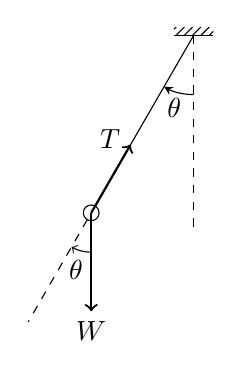
\begin{tikzpicture}

      \usetikzlibrary{patterns}
      % We define a tikz style which defines a fill pattern consisting of lines in the north east direction.
      % The draw=none option indicates that we do NOT want any stroke/border around the fill
      \tikzstyle{wall}=[fill,pattern=north east lines,minimum width=0.75cm,minimum height=0.3cm, draw=none]


      % Define dimensions and angles
      \def\hw{0.25}     % Half width of the small wall segment on top

      \def\angle{-120}  % Angle of string
      \def\r{2.5}         % Radius of string

      \def\br{0.1}      % Radius of bob

      \def\ar{0.75}      % Radius of the arc that represents the angle


      % Define coordinates used in the diagram
      \coordinate (bc) at (\angle:\r+\br);          % Center of the bob


      % Draw commands
      \draw (-\hw, 0) -- (\hw, 0);
      \draw [wall] (-\hw,0) rectangle (\hw,0.1);        % Draws a rectangle using the 'wall' pattern giving us the sloped lines

      \draw (0,0) -- (\angle:\r);       % string
      \draw [dashed] (0,0) -- (0,-\r);  % Dashed line down the middle

      \draw (bc) circle [radius=\br];        % The small circle representing the bob

      % Arc and symbol for the angle at the pivot
      \draw [->,>=stealth] (0, -\ar) arc (-90:\angle:\ar);
      \draw (-105:\ar+0.2) node {$\theta$};

      % Draw the two forces
      \draw [->,thick] (bc) -- ++(0,-1.25) node [below] {$W$};
      \draw [->,thick] (bc) -- ++ (\angle+180:1) node [anchor=south east, yshift=-5] {$T$};

      % Extend string using dashed line to show angle between vector W and the string
      \draw [dashed] (bc) ++ (\angle:\br) -- ++ (\angle:1.5);
      \draw [->] (bc) ++ (0,-0.5) arc (-90:\angle:0.5);
      \draw (bc) ++ (-105:0.75) node {$\theta$};

   \end{tikzpicture}
\end{center}


   Since for any angle $\theta \neq 0$ the two forces ($W$ and $T$) are not co-linear (pointing in the same or opposite directions) we need to resolve one of the forces in to its components. We choose to resolve $W$ parallel and perpendicular to the string.

   \tikzsetnextfilename{fbd2}
\begin{center}
   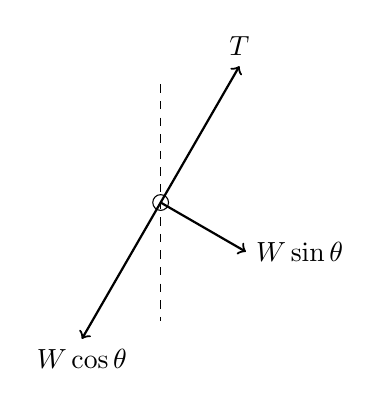
\begin{tikzpicture}

      % Definitions
      \def\angle{-120}  % Angle of string
      \def\br{0.1}      % Radius of bob
      \def\dh{1.5}      % Half-height of dashed line
      \def\lT{2}        % Length of the T and W cos theta vectors

      \coordinate (O) at (0,0);

      % Draw commands
      \draw (O) circle [radius=\br];
      \draw [dashed] (0,\dh) -- (0,-\dh);

      \draw [->, thick] (O) -- ++ (\angle:\lT) node [below] {$W \cos \theta$};
      \draw [->, thick] (O) -- ++ (\angle+180:\lT) node [above] {$T$};
      \draw [->, thick] (O) -- ++ (\angle+90:1.25) node [anchor=west] {$W \sin \theta$};

   \end{tikzpicture}
\end{center}


\section{Simple Harmonic Motion}

   Because of the tension in the string the bob cannot move in the radial direction (towards or away from the pivot along the direction of the string). This means that the tension exactly balances $W \cos \theta$ (the component of the weight parallel to the string). This leaves us with the component $W \sin \theta$ unbalanced. Therefore whenever $\theta \neq 0$ there is a net force acting on the bob which is pulling it towards the equilibrium position ($\theta = 0$ where the string is vertical, and $T$ and $W$ exactly balance each other).

   % A matrix of pendulum images representing the various stages in the motion of a simple pendulum

\tikzsetnextfilename{matrix}
\begin{center}
   \begin{tikzpicture}

       \usetikzlibrary{patterns}
       % We define a tikz style which defines a fill pattern consisting of lines in the north east direction.
       % The draw=none option indicates that we do NOT want any stroke/border around the fill
       \tikzstyle{wall}=[fill,pattern=north east lines,minimum width=0.75cm,minimum height=0.3cm, draw=none]

       % Define dimensions and angles
       \def\r{2.5}
       \def\hw{0.25}     % Half width of the small wall segment on top
       \def\br{0.1}      % Radius of bob
       \def\ar{0.75}      % Radius of the arc that represents the angle
       \def\hsangle{30}        % Half angle of the arc through which the pendulum swings (on either side of the vertical)

       \newcommand{\pendulum}[3]
       {
            % #1: Angle of pendulum string from x-axis
            % #2: Length of velocity vector (in cm). Negative values will cause vectors to point from RTL
            % #3: Image caption (displayed at bottom)

            \def\angle{#1}

           % Define coordinates used in the diagram
           \coordinate (bc) at (\angle:\r+\br);          % Center of the bob

           % Draw commands
           \draw (-\hw, 0) -- (\hw, 0);
           \draw [wall] (-\hw,0) rectangle (\hw,0.1);        % Draws a rectangle using the 'wall' pattern giving us the sloped lines

           \draw (0,0) -- (\angle:\r);       % string

           \ifnum \angle=-90                % Dashed line is NOT to be drawn when the angle is 90 since it overlaps with the string
           \else
               \draw [dashed] (0,0) -- (0,-\r);  % Dashed line down the middle.
           \fi

           \draw (bc) circle [radius=\br];        % The small circle representing the bo
           \draw [black!60] (-90-\hsangle:\r+\br) arc (-90-\hsangle:-90+\hsangle:\r+\br);       % An arc representing the path of the bob

           % We branch based on the value of #2 (the length of the v vector passed in)
           % If #2 == 0cm then we do NOT draw the velocity vector
           % To test #2 we use \ifthenelse where the first argument is the condition, the second is executed on truth and the third on false
           % We use \lengthtest to compare possibly floating point values. Note the explicit 'cm' added after #2 to cast it as a length and not a number.
            \ifthenelse{\lengthtest{#2 cm = 0cm}}{}{

                \draw [->, thick] (bc) -- ++ (\angle+90:#2);       % The velocity vector is tangential to the string so we rotate the angle by 90 degrees by adding 90 to the angle
            }

           \node [anchor=north, align=center, text width=4cm] at (-90:{\r + 0.35}) {#3};
           % align=center aligns the text horizontally
           % anchor=north ensures that the node starts below the specified point. This makes it aligned to the top vertically.
       }

       \matrix[row sep=0.5cm]
       {
            \pendulum{-120}{0}{(1) At maxima speed is zero} & \pendulum{-105}{0.3}{(2) Speed increasing} & \pendulum{-90}{0.5}{(3) At equilibrium speed is maximum} & \pendulum{-75}{0.3}{(4) Speed decreasing}\\

            \pendulum{-60}{0}{(5) At maxima speed is zero} & \pendulum{-75}{-0.3}{(6) Speed increasing in opposite direction} & \pendulum{-90}{-0.5}{(7) At equilibrium again. Maximum speed in opposite direction} & \pendulum{-105}{-0.3}{(8) Speed decreasing}\\
       };

   \end{tikzpicture}
\end{center}


   This unbalanced force causes the bob to accelerate towards the equilibrium position with its speed increasing. When the bob arrives at the equilibrium position the two forces are in balance and the net acceleration is zero but it is now moving with non-zero speed. This means it cannot stay in the equilibrium position and must continue to swing. As it swings to the other side the unbalanced force $W \sin \theta$ reappears but now it is pointing in the opposite direction (still towards the equilibrium position). This force causes the bob to slow down. Eventually its speed becomes zero and it comes momentarily to rest. This position is known as the maxima. The angle corresponding to the maxima is known as the amplitude.

   Since the maxima corresponds to a non-zero angle $\theta$ there exists an unbalanced force pulling towards the equilibrium position. This causes the bob to now move back towards the equilibrium position with increasing speed. Once again it arrives at the equilibrium position with non-zero speed and now moving in the opposite direction. Once again it flies past the equilibrium position and its speed is slowed down by $W \sin \theta$ acting towards the equilibrium position. When its speed becomes zero it achieves maxima in the opposite direction and will start to move back.

   The bob has now completed one cycle or oscillation. Because of the unbalanced force $W \sin \theta$ and the non-zero speed at the equilibrium position the bob is forced to repeat this motion over and over again. This is a type of simple harmonic motion. The bob is said to be performing oscillations. It can be shown that it takes the bob the same amount of time to complete a single oscillation regardless of the amplitude (how far the maxima is from the equilibrium position - as long as the amplitude is small). This is known as the \textbf{Time Period} of the oscillation.

\section{Time Period}

   It can be shown that the time period of a simple pendulum only depends upon the length of the string and strength of the force of gravity.
   %
   \beq
      T = 2 \pi \sqrt{\frac{l}{g}}
   \eeq
   %
   This makes pendulums very useful as time-keepers. As long as the length of the string remains fixed the pendulum takes the same amount of time for each oscillation and can be depended upon to keep time.
